% =====================================================================
%  ECT_summary.tex   (v7)
%  Mechanism-First Overview for Critical Review (English, ~17 pp)
%  Companion to:
%    Preprint:   doi:10.5281/zenodo.18917929
%    Companion:  doi:10.5281/zenodo.19430795
% =====================================================================
\documentclass[11pt,a4paper]{article}

\usepackage[T1]{fontenc}
\usepackage[utf8]{inputenc}
\usepackage{lmodern}
\usepackage[a4paper,margin=2.4cm]{geometry}
\usepackage{microtype}
\usepackage{amsmath,amssymb}
\usepackage[hidelinks]{hyperref}
\usepackage{setspace}
\usepackage{enumitem}
\usepackage{titlesec}
\usepackage{graphicx}
\usepackage[font=small,labelfont=bf]{caption}
\usepackage{xcolor}
\usepackage{longtable,booktabs,array}
\usepackage{float}
\usepackage{placeins}
\usepackage{tcolorbox}
\tcbuselibrary{skins,breakable}
\usepackage{tikz}
\usetikzlibrary{positioning,arrows.meta}

\setstretch{1.08}
\setlength{\parskip}{0.45em}
\setlength{\parindent}{0pt}

\titleformat{\section}{\large\bfseries}{\thesection.}{0.6em}{}
\titleformat{\subsection}{\normalsize\bfseries}{\thesubsection.}{0.5em}{}

\hypersetup{
  pdftitle={Euclidean Condensate Theory — Mechanism-First Overview},
  pdfauthor={Valeriy Blagovidov},
  pdflang={en}
}

\newtcolorbox{mechbox}[1][]{
  enhanced, breakable,
  colback=gray!4, colframe=gray!55,
  boxrule=0.4pt, arc=2pt,
  left=8pt, right=8pt, top=4pt, bottom=4pt,
  fonttitle=\bfseries,
  before skip=6pt, after skip=8pt,
  #1
}

\newcommand{\statA}{\textbf{Level~A}}
\newcommand{\statB}{\textbf{Level~B}}
\newcommand{\statC}{\textbf{Level~C}}
\newcommand{\statO}{\textbf{Open}}

\title{\textbf{Euclidean Condensate Theory (ECT):\\
A Concise Mechanism-First Overview}}

\author{Valeriy Blagovidov\thanks{Correspondence:
\texttt{blagovidov@phystech.edu},
\texttt{vblagovidov@gmail.com}.\,
ORCID: \href{https://orcid.org/0009-0008-6707-7068}{0009-0008-6707-7068}.}}
\date{June 2026}

\begin{document}
\maketitle

\begin{abstract}
\noindent
Euclidean Condensate Theory (ECT) studies whether Lorentzian
spacetime, coherent quantum dynamics, an effective gravitational
sector, and selected galactic and cosmological phenomenology can
arise as sector-dependent descriptions of a single ordered phase:
a real scalar medium $\Phi$ on a four-dimensional Euclidean
carrier with spontaneous symmetry breaking
$O(4)\!\to\!O(3)$.
The central claim is architectural: structures usually postulated
separately may instead appear as different regimes of one broken
branch.
This document is a concise mechanism-first entry point for
physicists who want the main construction, the principal results,
the status level of each headline claim (Level~A/B/C/Open), and
the most relevant tests without starting from the full preprint.
The colour sector is treated separately: exact local $SU(3)$
requires the additional completion postulate~P7 and does not belong
to the minimal $O(4)$-ordered condensate alone.
The full preprint is available at
\href{https://doi.org/10.5281/zenodo.18917929}{doi:10.5281/zenodo.18917929}
and the narrative companion at
\href{https://doi.org/10.5281/zenodo.19430795}{doi:10.5281/zenodo.19430795}.
\end{abstract}

% =====================================================================
\section{Introduction: from a Euclidean medium to observed physics}
\label{sec:intro}
% =====================================================================

The purpose of Euclidean Condensate Theory (ECT) is to test whether
several structures that today are introduced separately in
fundamental physics can arise from one underlying ordered phase.
Time, the causal cone, the Lorentzian metric, the quantum
description of coherent matter, and the gravitational sector are
usually layered on top of one another through independent
postulates. ECT proposes that they may instead be the effective
description of a single broken phase of a more primitive structure
that itself contains no time, no metric, and no quantum language.

The candidate primitive structure is intentionally minimal.
It is a four-dimensional Euclidean carrier on which a single real
scalar medium $\Phi$ is defined.
At this level the medium is pre-physical: it has no notion of
energy, no Planck constant, and no preferred direction.
A short list of structural properties specifies what the medium
admits — connectedness, directional isotropy under four-dimensional
rotations, local regularity with admissible defect submanifolds,
the existence of ordered configurations, and the recognition that
internal coordinates of the ordered branch are descriptive
redundancies rather than physical observables.

The central structural step of ECT is the appearance of an ordered
ground state in which the gradient of $\Phi$ acquires a
non-vanishing expectation value along one of the four Euclidean
directions.
The full four-dimensional rotational symmetry is broken down to its
three-dimensional subgroup; one direction becomes distinguished.
The analogy with ordering transitions in superfluid helium-3-A and
with gradient-condensate phases of Bose--Einstein systems is
methodological, not an identification: ECT places this kind of
mechanism at the foundational layer rather than as an emergent
material-physics effect on top of a pre-existing spacetime.

The broken phase carries two qualitatively distinct families of
disturbances.
Smooth single-valued disturbances of the collective phase form a
\emph{coherent sector}: they admit a partial reconstruction of the
standard quantum formalism through a topological action scale and a
reflection-positivity bridge, and they yield a recovery of
Schr\"odinger-type evolution in a stationary coherent regime.
Slowly varying disturbances of the ordered background motivate a
geometric/orientation extension.  The controlled equation used here is the
scalar-only metric equation.  A physical orientation stress
$T^{(n)}_{\mu\nu}$ requires a separately specified covariant
$S_n[g,n,\lambda_n]$; current anisotropic tensors are external proxies and
the orientation contribution remains Open.
In the galactic and cosmological applications, the same ordered
branch is then extended to an infrared critical-response regime
that organises the asymptotic phenomenology of galactic rotation
curves and contributes to a diagnostic-level multi-probe
cosmological compatibility layer.

In this picture Lorentzian spacetime, quantum coherence, and
gravity appear as sector-dependent regimes of one ordered medium
rather than as unrelated starting axioms.
ECT is therefore organised as a common ordered-medium architecture
with a separately tracked level of rigour for each sector.
The colour gauge sector lies outside the minimal four-dimensional
ordered structure and is introduced later through a distinct
internal-completion layer.

This overview is meant to function as a working map of mechanisms,
claims, status levels, and falsifiers.
Its purpose is to let a reader identify quickly which parts are
structural derivations, which parts depend on matching or closure
assumptions, and which parts remain open.
The four-level discipline introduced in
\S\ref{sec:status_discipline} keeps those categories explicit
throughout the document.

\paragraph{How to read this overview.}
A reader interested in the conceptual architecture should read
\S\S\ref{sec:intro}--\ref{sec:logic}.
A reader interested in testable phenomenology should start with
\S\S\ref{sec:cosmology}--\ref{sec:falsifiers}.
A reader interested in possible failure modes should go directly
to \S\S\ref{sec:falsifiers}--\ref{sec:status_map}.
The full preprint and the narrative companion
(links in \S\ref{sec:resources}) contain the technical derivations
underlying every claim made here.

% =====================================================================
\section{Scope of the framework: claims, open points, and current boundaries}
\label{sec:scope}
% =====================================================================

\textbf{The seven structural claims of ECT}, stated at the level of
mechanism rather than formula:

\begin{enumerate}[leftmargin=1.4em,itemsep=2pt]
\item Lorentzian spacetime and a single universal low-energy causal
      cone, whose effective speed is determined by the anisotropic
      stiffness of the ordered branch
      (\statA{} for cone emergence within the broken phase;
      \statB{} for matching the emergent cone speed to the
      observed vacuum speed of light).
\item Coherent quantum sectors with a pre-quantum topological action
      scale identified with Planck's constant at matching level
      (\statB), and a partial reconstruction of standard quantum
      formalism through reflection positivity and the
      Osterwalder--Schrader bridge; the spin--statistics
      connection holds at \statA{} for the free coherent kernel
      through the same Euclidean route.
\item A controlled scalar-only metric equation inside the declared
      ansatz, with matching to Newtonian gravity tracked separately
      (\statB{} within the scalar ansatz).  A physical orientation stress
      requires covariant $S_n[g,n,\lambda_n]$ and remains \statO{};
      $\mathcal X^{\rm cand}_{\mu\nu}$ is an external proxy only.
\item A \statA{} structural decoupling of the \emph{direct}
      classical cosmological-constant baseline channel through an
      emergent unimodular mechanism on the ordered branch.
      This is a structural removal of the direct-channel
      catastrophe, \emph{not} a derivation of the observed late-time
      value of $\rho_\Lambda$.
\item Galactic phenomenology from a specified interpolation fit
      (\statC{}), with the slope-four BTFR relation following
      algebraically only after the deep branch is assumed
      (\statB{}/\statC{}).  The provisional $\psi_\chi$ one-loop result
      does not derive the $\phi_u$ AQUAL branch; the coordinate bridge,
      environment law, and UDG/cluster interface remain \statO{}
      (\S\ref{sec:galactic}).
\item A retained five-probe cosmological consistency band for a
      single diagnostic deformation parameter at one~$\sigma$
      (\statC{}, presented explicitly as a multi-channel consistency
      diagnostic and not as a first-principles prediction).
\item A separately postulated $SU(3)$ colour-completion layer
      (postulate~P7), introduced because exact local $SU(3)$
      cannot be obtained from the minimal four-dimensional ordered
      condensate alone.
\end{enumerate}

\textbf{Current open points of ECT}
(tracked as \statO{} unless noted otherwise):

\begin{itemize}[leftmargin=1.4em,itemsep=2pt]
\item A strict first-principles theorem for the Born rule and the
      single-outcome side of the measurement problem.
      ECT has a \statB{} conditional route to Born-type weights via
      the reflection-positivity / Osterwalder--Schrader (RP/OS)
      Hilbert construction and a Gleason-type argument, once three
      reduced-description assumptions are admitted:
      C1, decohered alternatives carry an effective
      Hilbert/projector structure; C2, those alternatives are
      approximately orthogonal; and C3, probabilities add across
      mutually exclusive alternatives.
      Deriving C1--C3 from the bare ECT postulates, and resolving
      the single-outcome and measurement-update problem, remain
      \statO{}
      (see \S\ref{sec:quantum}).
\item Bell-type correlations, the no-signalling condition, and
      the Tsirelson bound are not derived from the present ECT
      structure; non-factorisable coherent correlations have a
      structural \statA/\statB{} route, but a full Bell/CHSH
      derivation is \statO.
\item The full low-energy quantum-field-theoretic architecture —
      strict locality, cluster decomposition, analyticity,
      crossing, and S-matrix theory — has not been re-derived
      from the ordered-medium formulation; matching is at the
      effective-action level only.
\item A first-principles derivation of the observed late-time
      value of the cosmological constant.
      ECT removes the direct vacuum-baseline channel, but the
      observed value remains a separate \statC/\statO{}
      determination problem.
\item A dynamical derivation of the ordered branch itself from
      the bare action (gradient condensation, OP-grad).
      In the current preprint this programme is decomposed into
      three recorded subproblems, and the remaining gap is
      localised to a single constraint-relaxation /
      coarse-graining bridge; the candidate bridges analysed so
      far do not close that gap, so the step remains \statO.
\item Derivation of hypercharge assignments, the full observed
      electric-charge spectrum, the flavour structure, the
      CKM/PMNS mixing matrices, and the three-generation hierarchy
      of the Standard Model.
\item Solution of the strong-CP problem: the topological coupling
      $\Theta(\phi)F\tilde F$ \emph{reopens} the problem within ECT
      rather than resolving it.
\item A predictive QCD-like phenomenology from the colour
      completion: at constant background couplings the P7-layer is
      structurally classificatory rather than predictive.
\item A predictive environment law closing the galactic interface
      across UDG, dwarf, and bullet-cluster matched-pair stress
      tests (central operational gap).
\item A finished ultraviolet completion of all sectors.
\end{itemize}

ECT is therefore best read as a structured theoretical framework
with a defined core, explicit matching layers, and a finite list of
open dependencies.
Every positive result below is presented with an explicit status
badge and a locator into the full preprint.

% =====================================================================
\section{Architecture of the model}
\label{sec:architecture}
% =====================================================================

ECT is built on three structural layers.

\textbf{S-layer (ontology of the $\Phi$-medium).}
Ten properties S1--S10 describe the $\Phi$-medium in purely
geometric and configurational terms, prior to any ordering, energy,
or quantum language:
connected four-dimensional Euclidean carrier (S1);
$O(4)$-directional isotropy (S2);
point homogeneity (S3);
local regularity with admissible defect submanifolds (S4);
locality (S5);
multiplicity of admissible configurations (S6);
admissibility of ordered states with
$\langle\partial_A\Phi\rangle\neq 0$ (S7);
medium character with pointwise internal coordinates as
descriptive redundancies (S8);
inhomogeneity of ordering (S9);
topological completeness (S10).
Because the $\Phi$-medium is pre-physical, no energy or
quantum-fluctuation language is used at this layer.

\textbf{Variational principle (DP).}
Physically realisable configurations extremise a local Euclidean
functional $S_E[\Phi]$ compatible with the basic symmetries of the
medium, with conditions ensuring well-posedness.

\textbf{Working postulates P1--P6.}
The minimal concrete realisation:
\begin{description}[leftmargin=1.4em,itemsep=2pt]
\item[P1] Connected four-dimensional Euclidean arena
      $\mathcal{M}^4$, $ds^2_E=\delta_{AB}dX^AdX^B$, with no
      distinguished time coordinate.
\item[P2] $O(4)$-invariant fundamental action,
      $S_E[\Phi]=S_E[\Lambda\cdot\Phi]$ for $\Lambda\in O(4)$.
\item[P3] Real scalar field $\Phi(X)$ with minimal local
      micro-action
      $S_E^{\rm bare}=\int d^4X\,[\tfrac{1}{2}(\partial_A\Phi)^2
        + V(\Phi)]$,
      $V=-\tfrac{\mu^2}{2}\Phi^2+\tfrac{\lambda}{4}\Phi^4$.
      The double-well is a $\mathbb{Z}_2$ structure, not a
      ``Mexican-hat''.
\item[P4] Physically relevant vacuum belongs to an ordered branch
      with $\langle\partial_A\Phi\rangle=u_0\,\delta_{Aw}$,
      $u_0>0$, selecting a preferred direction $w$ and breaking
      $O(4)\to O(3)$.
\item[P5] Pointwise internal coordinates of the ordered branch
      (phase $\theta(X)$, orientation $n_A(X)$) are descriptive
      redundancies; physical observables depend only on
      invariant gradient and holonomy data.
      The passage from P5 to the local gauge-structure route
      associated with $SU(2)\times U(1)$ is treated as a derived
      structural route on the smooth coherent branch, not as an
      independent postulate.
\item[P6] Multiplicity of admissible configurations and
      admissibility of non-uniform ordering (domains, transitions,
      defects).
\end{description}

\textbf{Derived branch rule (BR1).}
On the smooth coherent sector of the ordered branch the effective
order parameter is $\Phi_{\rm eff}=\rho\,e^{i\theta}$, $\rho>0$.
For closed contours not intersecting defect cores,
\begin{equation}
  \label{eq:winding}
  \oint_{\mathcal C}\partial_A\theta\,dX^A = 2\pi n,
  \qquad n\in\mathbb{Z},
\end{equation}
and the elementary coherent loop introduces the pre-quantum
topological action scale
\begin{equation}
  \label{eq:loop_action}
  S_{\rm loop,min}=2\pi S_0,
\end{equation}
where $S_0$ is the ECT precursor of $\hbar$ (matching: \statB).
BR1 is \emph{derived}: it follows once one restricts attention to
a smooth single-valued collective phase field on the broken phase.

\textbf{P7 is not part of the minimal architecture.}
Postulate~P7 (rank-3 complex internal module with Hermitian form
and fixed complex volume form, yielding exact local~$SU(3)$) is a
separate \emph{reverse-engineered} layer, introduced in Part~IV of
the preprint, and is required because $\mathfrak{su}(3)\not\subset
\mathfrak{so}(4)$: the colour sector cannot reside inside the
$O(4)$ ordered condensate alone. P7 is therefore additive to,
not part of, the P1--P6 core.

\textbf{Two energy scales and a separate length.}
The energy-dimension quantities are
$\phi_0\sim\bar M_{\rm Pl}$ and $v_2\approx246$~GeV.
The gradient amplitude $u_0=|\langle\partial_A\Phi\rangle|$ has
dimension GeV$^2$, with only the conditional dimensional estimate
$u_0\sim\phi_0m_\sigma$.  Separately,
$L_{\rm gal}=r_*=\sqrt{G_NM_{\rm bar}/g_\dagger}$ is a length inside
the adopted Level-C galactic functional, not a third energy amplitude;
its ECT matching is Open.  The logarithm
$\mathcal I_{\rm EW}=\ln(\phi_0/v_2)\approx36.8$ organises the Open
electroweak scale-generation programme.

% =====================================================================
\section{Input economy and structural reframings}
\label{sec:input_economy}
% =====================================================================

ECT spends its assumptions on a small microscopic layer
(\S\ref{sec:architecture}) and proposes structural routes to several
sectors that are usually treated as independent inputs in
fundamental physics. The two compact summaries below replace a long
audit table: a reader who wants more detail will find it in the
corresponding sections.

\begin{mechbox}
\textbf{Input audit.}
ECT does not claim that fewer assumptions prove the theory; the
point is to make explicit where assumptions are spent and where
reconstruction is claimed.
\begin{itemize}[leftmargin=1.2em,itemsep=1pt]
\item \textbf{Minimal ordered-medium input:}
      $\Phi$-medium on $\mathcal{M}^4$, variational principle DP,
      working postulates P1--P6, derived branch rule BR1.
\item \textbf{Recovered or structurally reconstructed:}
      Lorentzian causal cone; effective metric and orientation
      sector; coherent quantum branch; compact-$U(1)$ Abelian
      charge lattice; direct cosmological-constant channel
      decoupled.
\item \textbf{Matched / induced to standard low-energy physics:}
      $c\equiv c_*$, $\hbar\equiv S_0$, $G_N=c_*^4/(8\pi M_G^2)$,
      the energy scales $\phi_0,\,v_2$; and the distinct
      dimension-two gradient amplitude $u_0$.  The galactic
      $L_{\rm gal}$ is a Level-C closure length, not a matched energy scale.
\item \textbf{Closure / diagnostic layers:}
      the retained cosmological $\varepsilon$-band and late-time
      infrared scaling.  A galactic environment/history law $\Xi$
      is an Open future hypothesis, not an implemented closure.
\item \textbf{Separately postulated:}
      P7 (rank-3 complex internal module) for exact local
      $SU(3)$.
\item \textbf{Open:}
      dynamical origin of the ordered branch itself
      (gradient condensation, OP-grad);
      full first-principles Born theorem and the
      single-outcome/measurement-update problem;
      independent derivation of the reduced-description
      assumptions C1--C3 (\S\ref{sec:quantum});
      Bell/CHSH and the Tsirelson bound;
      the full low-energy QFT architecture (locality,
      cluster decomposition, analyticity, crossing,
      S-matrix);
      the observed value of $\rho_\Lambda$;
      hypercharge and the full Standard-Model
      charge/flavour/generation spectrum;
      the strong-CP problem within the CP-odd topological
      coupling;
      a finished UV completion.
\end{itemize}
\end{mechbox}

\textbf{Structural reframings, not final solutions.}
ECT does not present the following items as solved at the same
level. The point is to identify where the same ordered-medium
architecture gives a structural reframing and where the open
dependencies remain:

\begin{itemize}[leftmargin=1.4em,itemsep=2pt]
\item \textbf{Problem of time.}
      Time appears as an ordered-branch direction and effective
      parameter on the broken phase; the full quantum-gravity
      problem of time is not automatically solved.
\item \textbf{Quantum--classical boundary.}
      Coherent vs.~decohered/orientation sectors as a structural
      criterion; the strict measurement / single-outcome problem
      remains \statO.
\item \textbf{Born rule.}
      \statB{} conditional RP/OS + Gleason route given
      assumptions C1--C3 (\S\ref{sec:quantum});
      a derivation of C1--C3 from bare P1--P6 and the
      single-outcome / update problem remain \statO.
\item \textbf{Cosmological-constant catastrophe.}
      The direct vacuum-baseline channel decouples at \statA{}
      through the ordered-branch fixed kinetic determinant;
      the observed value of $\rho_\Lambda$ remains \statC/\statO.
\item \textbf{Galactic dark sector.}
      The adopted interpolation provides Level-C RAR/rotation-curve
      fits; slope-four BTFR is conditional B/C algebra inside that
      functional.  Scalar-to-galactic matching, $\Xi$, and the
      UDG/cluster interface remain \statO.
\item \textbf{Black-hole information.}
      Critical-shell / reduced-state mapping onto the islands /
      quantum-extremal-surface language;
      a complete Page-curve computation within ECT remains
      \statO.
\item \textbf{Gauge / colour sector.}
      Compact-$U(1)$ Abelian lattice and chiral $SU(2)$ structural
      routes from the broken phase;
      exact local $SU(3)$ via the separate postulate~P7;
      full SM charge/flavour/generation spectrum, confinement, and
      the strong-CP problem remain \statO.
\end{itemize}

The point of this section is not to prove ECT by parsimony, nor
to present a list of paradoxes resolved. It is to make explicit
where ECT spends assumptions and where it claims reconstruction;
the status labels remain the controlling standard.

% =====================================================================
\section{Claim-status discipline}
\label{sec:status_discipline}
% =====================================================================

Every quantitative or qualitative result in ECT is tagged with one
of four status levels. This taxonomy is used throughout the
preprint and is applied uniformly below.

\begin{description}[leftmargin=1.4em,itemsep=2pt]
\item[\statA] Strict structural or theorem-level derivation within
      stated assumptions. Example: emergent unimodular decoupling
      of the direct vacuum-baseline channel; Lorentzian cone
      emergence within the broken phase under the stated
      anisotropic-stiffness conditions.
\item[\statB] Conditional or closure-level derivation; a structural
      route exists, but at least one matching, calibration, or
      effective-functional step is required to obtain a number.
      Example: Level-B matching $S_0\leftrightarrow\hbar$; the BTFR
      slope as conditional B/C algebra inside adopted Level-C
      functional G; and the B/C comparison ansatz
      $g^\dagger_0\sim cH_0/(2\pi)$.
\item[\statC] Phenomenological or diagnostic consistency layer.
      Example: the retained five-probe effective band
      $\varepsilon\in[0.0296,0.0376]$ at $1\sigma$.
      This is empirical compatibility, not a first-principles
      prediction.
\item[\statO] Explicitly unresolved. Example: the strict
      first-principles Born theorem and the single-outcome
      problem; the observed value of $\rho_\Lambda$; the full
      Standard-Model charge, flavour, and generation structure;
      the strong-CP problem in the CP-odd topological sector;
      the environment law~$\Xi$.
\end{description}

The status discipline is asymmetric on purpose: weakening a result
from \statA{} to \statB{} is admissible if a derivation step is
found to be incomplete; strengthening in the other direction is
not permitted without an explicit rigorous derivation.

% =====================================================================
\section{Derivation logic and mechanism map}
\label{sec:logic}
% =====================================================================

The architecture of \S\ref{sec:architecture}, the input audit of
\S\ref{sec:input_economy}, and the status discipline of
\S\ref{sec:status_discipline} together generate a single mechanism
flow that is the subject of the remainder of this overview.
Figure~\ref{fig:logic} summarises it.

\begin{figure}[h]
\centering
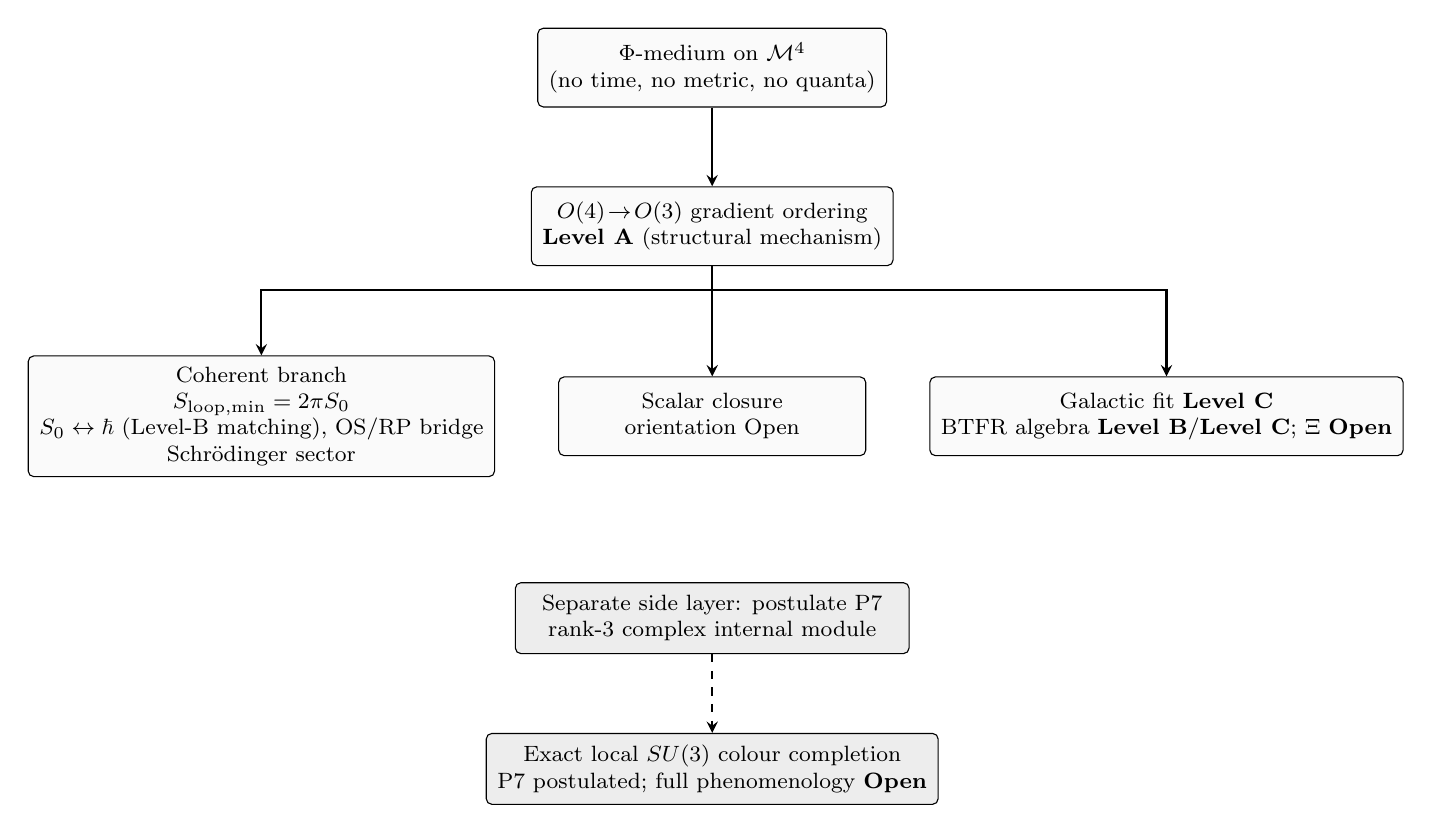
\begin{tikzpicture}[
  node distance=10mm and 8mm,
  every node/.style={font=\footnotesize},
  box/.style={draw, rounded corners=2pt, align=center,
              inner sep=4pt, minimum width=3.9cm,
              minimum height=1.0cm, fill=gray!4},
  side/.style={draw, rounded corners=2pt, align=center,
              inner sep=4pt, minimum width=5.0cm,
              minimum height=0.9cm, fill=gray!14},
  arr/.style={->, thick, >=stealth},
  outarr/.style={->, thick, >=stealth, dashed}
]

\node[box] (medium)
  {$\Phi$-medium on $\mathcal{M}^4$\\
   (no time, no metric, no quanta)};

\node[box, below=of medium] (ordered)
  {$O(4)\!\to\!O(3)$ gradient ordering\\
   \statA{} (structural mechanism)};

\node[box, below=14mm of ordered] (geom)
  {Scalar closure\\
   orientation Open};

\node[box, left=of geom] (coh)
  {Coherent branch\\
   $S_{\rm loop,min}=2\pi S_0$\\
   $S_0\leftrightarrow\hbar$ (Level-B matching), OS/RP bridge\\
   Schr\"odinger sector};

\node[box, right=of geom] (ir)
  {Galactic fit \statC\\
   BTFR algebra \statB/\statC; $\Xi$ \statO};

\draw[arr] (medium) -- (ordered);
\draw[arr] (ordered.south) -- ++(0,-3mm) -| (coh.north);
\draw[arr] (ordered) -- (geom);
\draw[arr] (ordered.south) -- ++(0,-3mm) -| (ir.north);

\node[side, below=16mm of geom] (p7)
  {Separate side layer: postulate P7\\
   rank-3 complex internal module};

\node[side, below=of p7] (su3)
  {Exact local $SU(3)$ colour completion\\
   P7 postulated; full phenomenology \statO};

\draw[outarr] (p7) -- (su3);

\end{tikzpicture}
\caption{Simplified derivation logic of ECT. Arrows show mechanism
flow, not equal-strength theorem statements. The $SU(3)$ branch is
separate because it requires P7 rather than following from the
minimal $O(4)$-ordered medium; Born-type weights are part of the
conditional quantum-reconstruction layer discussed in
\S\ref{sec:quantum}.}
\label{fig:logic}
\end{figure}

The same flow is expressed verbally as five structural routes from
one medium to qualitatively distinct phenomena:

\begin{enumerate}[leftmargin=1.4em,itemsep=2pt]
\item \textbf{Ordered branch} (P4, anisotropic kinetic tensor with
      $\alpha>\beta$): selection of a Lorentzian causal cone and an
      effective signature $(-,+,+,+)$.
      \S\ref{sec:cone}.
\item \textbf{Smooth coherent sector} (BR1, smooth single-valued
      $\theta$): integer winding,
      $S_{\rm loop,min}=2\pi S_0$, reflection positivity, and an
      Osterwalder--Schrader bridge yielding a \emph{partial
      Hilbert-space reconstruction route} for the coherent quantum
      sector. \S\ref{sec:quantum}.
\item \textbf{Scalar metric response and Open orientation extension}:
      the displayed equation is scalar-only.  A physical
      $T^{(n)}_{\mu\nu}$ requires covariant $S_n[g,n,\lambda_n]$;
      $\mathcal X^{\rm cand}_{\mu\nu}$ is only an external proxy.
      \S\ref{sec:gravity}.
\item \textbf{Specified galactic interpolation}: Level-C RAR/rotation
      fits and conditional BTFR algebra.  It is not derived by the
      provisional $\psi_\chi$ loop or by the scalar trace equation.
      A separate scalar-only diagnostic closure is used for cosmology.
      \S\S\ref{sec:cosmology}--\ref{sec:galactic}.
\item \textbf{Reverse-engineered colour layer} (P7, rank-3 complex
      internal module): exact local $SU(3)$ at the cost of a
      separate postulate beyond the $O(4)$-ordered condensate.
      \S\ref{sec:gauge}.
\end{enumerate}

% =====================================================================
\section{How ECT differs from nearby frameworks}
\label{sec:comparison}
% =====================================================================

ECT is not a recombination of existing programmes. The two tables
below locate ECT against the closest established or proposed
frameworks; the split into \emph{conceptual foundations}
(Table~\ref{tab:ect_vs_nearby_A}) and
\emph{phenomenology and gauge sector}
(Table~\ref{tab:ect_vs_nearby_B}) is for readability only.

\renewcommand{\arraystretch}{1.22}
\small
\begin{longtable}{@{}p{2.5cm} p{2.9cm} p{2.7cm} p{4.4cm} p{2.0cm}@{}}
\caption{Conceptual foundations.}
\label{tab:ect_vs_nearby_A}\\
\toprule
\textbf{Sector} & \textbf{Standard approach} &
\textbf{Nearby alternatives} & \textbf{ECT mechanism} &
\textbf{Status}\\
\midrule
\endfirsthead
\multicolumn{5}{@{}l}{\textit{Table~\ref{tab:ect_vs_nearby_A},
continued.}}\\
\toprule
\textbf{Sector} & \textbf{Standard approach} &
\textbf{Nearby alternatives} & \textbf{ECT mechanism} &
\textbf{Status}\\
\midrule
\endhead
\bottomrule
\endfoot

Spacetime signature
& Lorentzian metric assumed
& CDT~\cite{Ambjorn2005}, causal sets, analogue gravity;
  clock-field route~\cite{MukohyamaUzan2013}
& Ordered Euclidean branch selects an effective Lorentzian cone;
  formula and matching given in \S\ref{sec:cone}.
& \statA{} existence; \statB{} matching\\

Quantum formalism
& Hilbert space and Born rule postulated
& Many-worlds, Bohm, QBism, OS reconstruction
& Coherent branch gives an RP/OS route to Hilbert-space dynamics;
  Born-type weights remain conditional.
& \statB{} structural; Born thm.~\statO\\

Gravity
& Metric field fundamental
& Sakharov-induced gravity, Jacobson thermodynamic
  derivation~\cite{Jacobson1995},
  Einstein--aether/vector-tensor analogues~\cite{Jacobson2004},
  Verlinde entropic gravity~\cite{Verlinde2011}, analogue
  gravity~\cite{Volovik2003,Padmanabhan2010}
& Scalar metric ansatz; orientation Open.
& \statB{}; \statO{}\\

Cosmological constant
& Vacuum energy gravitates; demands cancellation $\sim 10^{120}$
& Unimodular gravity, sequestering, Weinberg no-go arguments
& Direct vacuum-baseline channel decouples through the
  ordered-branch fixed determinant; observed value remains
  diagnostic / open.
& \statA{} direct; observed $\rho_\Lambda$ \statC/\statO\\

\end{longtable}
\normalsize

\textbf{Related independent work on Lorentz-signature emergence.}
Mukohyama and Uzan studied the emergence of Lorentzian dynamics
from a four-dimensional Riemannian microscopic structure through
a clock-field derivative background~\cite{MukohyamaUzan2013}.
This is nearby prior work on emergent Lorentz signature, but it is
not the basis of ECT: the present construction uses a different
scalar-medium architecture, an ordered-gradient condensate, a
coherent/decohered branch split, and a different gravitational and
cosmological programme.

\renewcommand{\arraystretch}{1.22}
\small
\begin{longtable}{@{}p{2.5cm} p{2.9cm} p{2.7cm} p{4.4cm} p{2.0cm}@{}}
\caption{Phenomenology and gauge sector.}
\label{tab:ect_vs_nearby_B}\\
\toprule
\textbf{Sector} & \textbf{Standard approach} &
\textbf{Nearby alternatives} & \textbf{ECT mechanism} &
\textbf{Status}\\
\midrule
\endfirsthead
\multicolumn{5}{@{}l}{\textit{Table~\ref{tab:ect_vs_nearby_B},
continued.}}\\
\toprule
\textbf{Sector} & \textbf{Standard approach} &
\textbf{Nearby alternatives} & \textbf{ECT mechanism} &
\textbf{Status}\\
\midrule
\endhead
\bottomrule
\endfoot

Galactic dark sector
& Particle dark matter, NFW halos
& MOND/AQUAL~\cite{Milgrom1983,Famaey2012}, Verlinde emergent
  dark gravity
& Specified interpolation fit; BTFR slope~4 is conditional
  algebra inside its deep branch (\S\ref{sec:galactic}).
& fit \statC; slope \statB/\statC; $\Xi$ \statO\\

Hubble / $S_8$ tensions
& Parameter extensions to $\Lambda$CDM, EDE, modified gravity
& EDE, interacting DE, $f(R)$~\cite{Sotiriou2010},
  quintessence~\cite{Carroll2001}
& Single late-time deformation parameter $\varepsilon$;
  retained five-probe consistency band at $1\sigma$
  (\S\ref{sec:cosmology}).
& \statC{} consistency; first-principles \statO\\

Gauge sector / $SU(3)$
& Group assigned by the Standard Model
& GUTs, internal-geometry programmes
& Compact-$U(1)$ Abelian charge lattice (derived);
  chiral $SU(2)$ from the oriented broken phase;
  exact local $SU(3)$ via the separate postulate~P7.
& $U(1)$ \statA/\statB; $SU(2)$ \statB;
  $SU(3)$ via P7; full SM spectrum \statO\\

\end{longtable}
\normalsize

Three further differences merit explicit statement:
ECT \emph{does not} assume the existence of Lorentzian spacetime
anywhere as a fundamental ingredient;
the specified galactic fit contains no particle-halo term, without
excluding hidden-sector particles; the late-time closure likewise does not
take dark energy as an external fluid;
and ECT \emph{does not} resolve the strong-CP problem.

% =====================================================================
\section{Emergent spacetime and the universal cone}
\label{sec:cone}
% =====================================================================

In the broken phase, linearised excitations around the ordered
background propagate with an effective kinetic tensor that becomes
anisotropic in the direction $w$ selected by
$\langle\partial_A\Phi\rangle$.
For canonical anisotropic stiffness couplings $(\alpha,\beta)$ the
longitudinal/transverse split admits a Lorentzian signature window
if and only if $\alpha>\beta$, in which case the effective
low-energy cone has a single universal propagation speed:
\begin{equation}
  \label{eq:cstar}
  c_* = \sqrt{\beta/(\alpha-\beta)},
  \qquad
  \text{Lorentzian window: } \alpha>\beta.
\end{equation}

\begin{mechbox}
\textbf{Mechanism in ECT.}
$O(4)\!\to\!O(3)$ SSB of the gradient condensate selects a
preferred direction; the kinematic constraint $n^An_A=1$ on the
orientation variable, combined with $\alpha>\beta$, makes the
longitudinal mode disperse on a single emergent light cone.
Matching of $c_*$ to the observed vacuum speed $c$ is a separate
calibration step.\\
\textbf{What this establishes.} A concrete route from Euclidean
ordering to Lorentzian signature, an effective time direction, and
a universal low-energy causal cone within the broken phase.\\
\textbf{Status.} \statA{} for emergence of the cone within the
broken phase; \statB{} for identifying $c_*$ with the observed
$c$.\\
\textbf{Where in the full preprint.} Part~I, ordered-branch and
metric-classification sections; cone universality theorem.\\
\textbf{Falsifier.} An unsuppressed sector-dependent low-energy
propagation speed (e.g.~photon--graviton differences beyond the
GW170817 bound) would falsify universal-cone emergence.
\end{mechbox}

% =====================================================================
\section{Quantum sector: what is recovered and what remains open}
\label{sec:quantum}
% =====================================================================

ECT reconstructs the quantum sector on the coherent branch rather
than postulating Hilbert space at the foundational level.
The smooth coherent sector of the ordered branch supports a partial
reconstruction of the standard quantum formalism through the
Euclidean path-integral route, with reflection positivity providing
the Osterwalder--Schrader bridge to a Hilbert space and a unitary
evolution on the coherent stationary sector.
At the overview level the coherent-sector evolution is written
schematically as
\begin{equation}
  \label{eq:qs}
  iS_0\,\partial_t\Psi
  = \hat H_{\rm coh}\Psi
  + \Delta_{\rm dec}\Psi
  + \Delta_{\nabla}\Psi,
\end{equation}
where $\Delta_{\rm dec}$ denotes reduced-state / decoherence
corrections from the influence functional and $\Delta_{\nabla}$
collects higher-gradient corrections to the kinetic operator;
the explicit form of these correction operators is given in the
corresponding part of the full preprint and is not needed at the
overview level.
For coherent stationary eigenmodes
$\hat H_{\rm coh}\Psi=E\Psi$, $\Psi\sim e^{-i\omega t}$, this
yields $E=S_0\omega$ up to the controlled corrections.
The standard Planck--Einstein relation $E=\hbar\omega$ then follows
from the \statB{} matching $S_0=\hbar$.

\textbf{Born-type weights as a conditional reconstruction.}
ECT does not insert Born weights by fiat.
Instead, once the reduced coherent/decohered description reaches
three specific assumptions — C1: decohered alternatives admit an
effective Hilbert/projector structure; C2: those alternatives are
approximately orthogonal; C3: probabilities add across mutually
exclusive alternatives — the RP/OS Hilbert construction together
with a Gleason-type uniqueness argument selects the Born weights.
This conditional reconstruction has \statB{} status.
What remains open is earlier in the chain: deriving C1--C3
directly from the bare ECT postulates, obtaining a
first-principles Born theorem without these reduced-description
assumptions, and resolving the single-outcome /
measurement-update problem.
Common-medium nonfactorisation is a candidate \statB{}/\statO{} route;
the physical state/channel, Bell and no-signalling correlators, and
Tsirelson saturation remain \statO.

The spin--statistics connection is established at \statA{} for
the free coherent kernel through the Euclidean
Osterwalder--Schrader route (a L\"uscher--Osterwalder-class
argument verified against the original sources); the interacting
completion remains \statO.
The free antisymmetric kernel gives an exact mathematical Pauli/CAR
statement; applying it to physical interacting ECT matter remains
\statB{}/\statO{} pending the spinor/kernel completion.
A conditional CPT route is identified through the Euclidean
Osterwalder--Schrader framework; a preferred-direction operator
arises only as a CPT-odd branch-sensitive operator consistent with
the exact symmetry backbone.
PES-R provides a status-separated inventory of stationarity, pairwise
record, finite-time stability, and protocol diagnostics; it is not a
universal persistent-sector selection theorem.
PES is retained as a Level-B organising/filter framework, not as a
universal one-history action.  Its operational objects must remain separate:
the pairwise record/decoherence exponent $\Phi_{ab}(T)$, a declared
translation-susceptibility diagnostic $\Gamma_{\rm tr}[q;\eta]$, the decay
rate/width $\gamma_a$ (or $S_0\gamma_a$ in action units), and protocol entropy
production $\Sigma$.  None of these supplies a general mean-EOM variational
	additive action-plus-decoherence mean-EOM functional, and no universal
	forward/reverse probability law follows without a named protocol.  The ECT
	record-sector vertex, state, and
noise kernel remain Open/Not Identifiable.

\begin{mechbox}
\textbf{Mechanism in ECT.}
Reflection positivity and OS reconstruction on the coherent branch,
together with the topological pre-quantum scale
$S_{\rm loop,min}=2\pi S_0$.\\
\textbf{What this establishes.} A coherent-sector route to
Hilbert-space dynamics, the Schr\"odinger sector, and a
topological precursor of $\hbar$; Born-type weights follow once
the reduced-description assumptions C1--C3 are in place.\\
\textbf{Status.} \statB{} for the OS bridge, PES, and the
$S_0=\hbar$ matching; \statB{} conditional for Born-type weights
once assumptions C1--C3 are admitted; \statO{} for the
first-principles Born theorem from bare P1--P6, for C1--C3
themselves, and for the single-outcome / measurement-update
problem; \statA{} for the spin--statistics connection on the free
coherent kernel (interacting completion \statO).\\
\textbf{Where in the full preprint.} Part~III, sections on coherent
dynamics, PES, hybrid consistency, and the influence-functional
decoherence model, with the separately reviewed PES-R repair still
pending before the record-sector owner blocks become current.\\
\textbf{Discriminant.} Robust violation of the explicitly matched
coherent-sector quantum dynamics would constrain that closure. Present
gravity-decoherence and mediator-loophole bounds test external
comparator classes, not an absolute ECT rate: the ECT record vertex,
state, and noise kernel are Open/Not Identifiable.
\end{mechbox}

% =====================================================================
\paragraph{DP-02 negative spectral result.}
The tested minimal scalar vacuum channel has $J_\phi\propto\omega^3$;
the equal-mass Gaussian composite vacuum channel has
$J_{\mathcal O}\propto\omega^9$ with a finite-time $T^{-8}$ envelope; and
its thermal regime has $J_{\mathcal O}^{\rm th}\propto T_b^5/k$.  None gives
the universal Diósi--Penrose $1/k^2$ infrared form.  Alternative ECT
state/pole/vertex constructions remain Open.

\section{Gravity and the cosmological-constant catastrophe}
\label{sec:gravity}
% =====================================================================

The controlled metric equation in the displayed scalar-only
Jordan-frame ansatz is, in an undivided convention,
\begin{equation}
  \label{eq:gee}
  F\,G_{\mu\nu}
  = \frac{8\pi G_N}{c^4}\,T_{\mu\nu}
    + \mathcal{T}^{(q)}_{\mu\nu},
\end{equation}
where $\mathcal{T}^{(q)}_{\mu\nu}$ collects scalar derivative and
potential terms.  The factor $G_N/F$ appears only after all terms are
divided by $F$.  The displayed action contains no independent
orientation field and therefore does not derive
$T^{(n)}_{\mu\nu}$; $\mathcal X^{\rm cand}_{\mu\nu}$ is only an external
proxy.  A covariant $S_n[g,n,\lambda_n]$ and its metric variation remain
\statO.  Dividing the equation by $F$ introduces no orientation term.
The scalar audit uses $a=f_{,q}/f$,
$\mathcal A=K+3f_{,q}^2/(2f)$, and
$\mathcal E=V_{,q}-2aV-(a/2)\rho_{\rm m}$; at a stable homogeneous root,
$d\ln\bar f/d\rho_{\rm m}=a^2/(2\mathcal E_{,q})\ge0$ and
$m_{\rm loc}^2=\mathcal E_{,q}/\mathcal A$ are conditional local-response
statements, not finite-body screening.  The FRW/Hubble/JWST diagnostics use
the scalar-only background.  The Planck-scale matching
$G_N=c_*^4/(8\pi M_G^2)$ is kept as a separate matching relation.

M (the microscopic director operator), S (this Level-B scalar ansatz), and G (the adopted Level-C galactic functional) are distinct. M$\neq$S by operator content and S$\to$G is Open. The historical LOF appendix is a mixed branch audit: the heavy-radial proxy result does not select another coordinate or the galactic functional, and the matter-to-Lorentz-order map remains Open.

\textbf{The cosmological-constant catastrophe (direct channel).}
In a standard general-relativistic framework, the quartic
double-well baseline $V(\phi_0)=-\mu^4/(4\lambda)$ would gravitate
as a cosmological constant of order $\lambda M_{\rm Pl}^4/4$,
overshooting $\rho_\Lambda^{\rm obs}\sim(2.3\times 10^{-3}\,{\rm eV})^4$
by $\sim 10^{120}$. In ECT this catastrophe is removed at \statA{}
for the leading ordered-branch sector through an
\emph{emergent unimodular decoupling} theorem: the determinant of
the ordered-branch kinetic tensor is fixed by the kinematic
constraint $n^An_A=1$:
\begin{equation}
  \sqrt{-\det K^{AB}} = \beta^2/c_*,
\end{equation}
and consequently the bare baseline $V(\phi_0)$ does not source the
local emergent gravitational dynamics. Conditional on a one-line
spectral assumption on the full quadratic fluctuation operator
(condition~$H_\Lambda$), the zero-derivative one-loop vacuum
contribution is absorbed into the same fixed kinetic-determinant
structure. The direct $10^{120}$-level UV-to-IR cancellation
characteristic of the standard framework is therefore structurally
absent in the leading ordered-branch sector.
Two further strengthenings are recorded in the current preprint:
the decoupling statement is realised in an explicit exact FRW
ordered-branch background (the realisation-side tasks of the
cosmological-constant programme are completed), and an area-law
holographic entropy bound is established as a structural property
of the ordered medium (\statA{} for the scaling, \statB{} for
the coefficient).

\textbf{Remaining determination problem.} The observed numerical value
of $\rho_\Lambda$ remains a separate \statC{} determination problem;
the natural infrared scaling
$\rho_\Lambda\sim c_\Lambda M_{\rm Pl}^2 H_0^2$ with
$c_\Lambda=\mathcal{O}(1)$ is order-of-magnitude consistent but the
coefficient is not yet derived.

\begin{mechbox}
\textbf{Mechanism in ECT.}
Scalar-only metric response in the declared Jordan-frame ansatz;
fixed determinant of the ordered-branch kinetic tensor through
$n^An_A=1$ for the separate direct-channel decoupling result.\\
\textbf{What this establishes.} Consistent scalar-only metric
normalisation and a direct-channel decoupling of the vacuum baseline
in the leading ordered branch.  A covariant orientation-stress source
is not established by the displayed action.\\
\textbf{Status.} exact algebra within the declared Level-B scalar
ansatz for the metric normalisation; separately \statA{} for the
direct-channel decoupling theorem;
\statO{} for the orientation-stress extension; \statC{} for the
observed value of~$\rho_\Lambda$; \statO{} for the first-principles
value of~$c_\Lambda$.\\
\textbf{Where in the full preprint.} Part~II, sections on
generalised Einstein equations, the cosmological-constant problem,
and the decoupling theorem.\\
\textbf{Falsifier.} A robust demonstration that constant
vacuum-energy shifts source the local emergent gravitational
equations with standard GR strength would falsify the
direct-channel decoupling claim. Independently, a statistically
robust phantom crossing $w<-1$ would put the present
ordered-branch dark-energy closure under serious pressure.
\end{mechbox}

% =====================================================================
\section{Cosmology and current observational tensions}
\label{sec:cosmology}
% =====================================================================

The macroscopic ordered-branch closure admits a uniform effective
late-time deformation,
\begin{equation}
  \label{eq:eps_def}
  G_{\rm eff}(z)/G_N = (1+z)^{2\varepsilon},
\end{equation}
where $\varepsilon$ is a single diagnostic parameter of the
\emph{retained five-probe analysis layer} (Hubble plus sound
horizon $r_s$, JWST high-$z$ extraction, cosmic chronometers,
$f\sigma_8$ redshift-space distortions, integrated Sachs--Wolfe
cross-correlation). A common effective constraint from the five
retained probes yields
\begin{equation}
  \varepsilon\in[+0.0296,\,+0.0376] \quad (1\sigma), \quad
  [+0.021,\,+0.042] \quad (2\sigma).
\end{equation}
This is a \emph{consistency window} across observationally distinct
channels with different kernels and systematics.
It should be read as an indirect multi-channel
\emph{viability test} of the present effective parameterisation,
rather than yet as a global likelihood combination or a closed
first-principles derivation.

The associated age indicators of the Lorentzian branch are
$\sim 13.5$~Gyr under baseline-$H_0$ mapping and
$\sim 12.5$~Gyr under inferred-$H_0$ mapping; the JWST early-galaxy
sector contributes the binding lower edge of the retained band
under the present extraction pipeline.
Excluded probes are listed separately: BAO and lensing $A_{\rm lens}$
as methodology-limited under the uniform-$\varepsilon$ ansatz;
$S_8$~(KiDS-1000) and $\sigma_8$ from clusters as outside the
present $\varepsilon$-sector under a category-error interpretation;
the SN~Ia channel as non-independent of the retained anchors.

Within the same ordered-branch background, the late-time
dark-energy sector is a \emph{thawing} closure. The exact
background relation is $w_0=(r_0-1)/(r_0+1)$, where $r_0$ is the
present kinetic-to-condensate energy ratio
($r_0\approx 0.095$ at the calibrated benchmark), with the
linearised form $w(z)\simeq -1+2f_0\,e^{-\kappa z}$,
$f_0\approx 0.087$. The frequently quoted value
$w_0\approx -0.83$ is a DR1-anchored \emph{calibrated thawing
benchmark} (\statB): a useful reference point rather than a
derivation from the microscopic layer. The closure keeps
$w(z)\ge -1$ at all redshifts.

\begin{mechbox}
\textbf{Mechanism in ECT.}
A single ordered-branch deformation parameter $\varepsilon$
tracking the same condensate background that controls both the
dark-energy sector and the epoch-dependent baseline acceleration
scale $g^\dagger_{\rm bg}(z)=c_*H(z)/(2\pi)$.\\
\textbf{What this establishes.} A retained late-time consistency
window in which one effective deformation parameter organises
several observational channels at once.\\
\textbf{Status.} \statC{} consistency layer; first-principles
derivation of $\varepsilon(z)$ from the closure functions is
\statO.\\
\textbf{Where in the full preprint.} Part~II, retained five-probe
section and its methodological appendix.\\
\textbf{Falsifier.} A future joint analysis with the same retained
probes that stably pulls $\varepsilon$ below zero (in particular
through JWST high-$z$ extraction stabilising at a binding lower
edge $\varepsilon\le 0$) would put the present sector under
serious pressure.
\end{mechbox}

% =====================================================================
\section{Galactic phenomenology}
\label{sec:galactic}
% =====================================================================

In the deep low-acceleration regime of the adopted galactic closure
the asymptotic galactic field equation reduces to
$g\simeq\sqrt{g_N\,g_\dagger}$, and the asymptotically flat
rotation-curve velocity satisfies
\begin{equation}
  \label{eq:btfr}
  v_\infty^4 = G_N\,M_b\,g_\dagger.
\end{equation}
The asymptotic baryonic Tully--Fisher slope of $4$ is algebraic only
inside this specified deep-branch interpolation; the closure itself is not
derived from the corrected scalar action.  In particular,
$\phi_u=\beta_\phi^{-1}\ln(u/u_\infty)$ is distinct from
$\psi_\chi=\ln(\chi/\chi_{\rm vac})$, and the provisional
$K_\chi\propto e^{-\psi_\chi/2}$ loop does not derive the AQUAL branch.
The practical fit returns per-galaxy $g^\dagger_{\rm eff}$ values (Level~C).  The reference $g^\dagger_0\approx1.04\times10^{-10}$\,m/s$^2$ is a matched B/C benchmark, compared with the empirical $a_0\approx1.2\times10^{-10}$\,m/s$^2$; it is not a universal fit output.  A possible regression $g^\dagger_{\rm eff}/g^\dagger_0=\Xi(\rho_{\rm env},\bar\phi_{\rm env},\ldots)$ is an Open future hypothesis, not the current implementation.  The sample medians are $\chi_r^2\approx2.7$ (fixed $M/L$) and $\approx1.4$ (free $M/L$), versus the quoted MOND comparator $\approx3.1$ on comparable footing.  The conditional length $L_{\rm gal}=r_*=\sqrt{G_NM_b/g^\dagger}$ belongs to G and is not a condensate energy scale.  The physical S$\to$G map, particle content, and cosmological fraction budget remain Open.

The UDG inverse diagnostic now uses the Wolf coefficient~3 at
$R_{1/2}=4R_e/3$ and the unconstrained quantity
$\Xi_{\rm alg}=\mathcal R_{\rm dyn}(\mathcal R_{\rm dyn}-1)g_N/g^\dagger_0$.
It is a physical environment factor only when $\Xi_{\rm alg}\ge0$.
Central values are $-0.00369$ (DF4; no admissible nonnegative-$\Xi$
solution), $0.00516$ (FCC~224), $0.892$ (NGC~5846-UDG1), and $4.981$
(Dragonfly~44); DF2's dispersion bracket gives $0.031$--$0.423$.  The
previous logarithmic nuisance-parameter band is withdrawn; a full Jeans posterior
is Open.

The displayed force-dimensionality curve belongs to the separate
illustrative point-source law $\mu_{\rm dim}=x/\sqrt{1+x^2}$, not practical
G; an extended-galaxy extraction requires measured $p_N(r)$ and has not been
performed.  The cluster script is only an exact order/argmax-preservation
identity for hand-set maps.  It supplies no morphology/lensing evidence or
observed amplitude inference; a physical cluster response and likelihood
remain Open.

\begin{mechbox}
\textbf{Mechanism in ECT.}
Adopted low-acceleration interpolation closure; BTFR slope as
an algebraic corollary of its deep-branch limit; exploratory
future regression of per-galaxy $g^\dagger_{\rm eff}$ through a prespecified Open law~$\Xi$; the current fits do not implement it.\\
\textbf{What this establishes.} A Level~C fit benchmark and a
conditional algebraic BTFR slope inside the adopted closure; it does
not establish the physical $u\leftrightarrow\chi$ bridge or scalar
screening.\\
\textbf{Status.} BTFR slope \statB{}/\statC{} conditional on the closure; per-galaxy $g^\dagger_{\rm eff}$ fit outputs \statC{}; matched $g^\dagger_0$ reference \statB{}/\statC{}; the environment/history law~$\Xi$, UDG closure, and finite-body screening \statO.\\
\textbf{Where in the full preprint.} Part~II, sections on galactic
dynamics, radial acceleration relation, SPARC fits, and the UDG
stress-test appendix.\\
\textbf{Discriminant.} A robust BTFR slope inconsistent with $4$ would reject the adopted deep-branch closure.  Independently, a prespecified boundary-aware Jeans likelihood for the declared UDG sample tests that closure; failure rejects the closure, not ECT as a whole.  An unrestricted $\Xi$ family is not identifiable and is therefore not used as a falsifier.
\end{mechbox}

% =====================================================================
\section{Gauge sector and the SU(3) completion}
\label{sec:gauge}
% =====================================================================

On the smooth coherent branch the compact phase $\theta$ admits a
bundle covariance whose connection plays the role of an effective
$U(1)$ gauge field; integer winding around defect cores then
implies a compact-$U(1)$ Abelian charge lattice. The full
observed Standard-Model charge spectrum — including hypercharge,
flavour, and generation structure — is not derived from this
mechanism and remains \statO.
A recorded \emph{colour-interlock} consistency layer now
constrains completions: with the standard $\mathbb{Z}_6$-type
global quotient, hypercharge, colour and weak data must satisfy
an explicit congruence, which fixes the fractional electric
pattern per colour class ($Q\equiv -t/3 \pmod 1$) and reduces
the residual freedom to an explicitly characterised discrete
family — a consistency requirement on completions, not a
derivation.
A chiral $SU(2)$ sector is structurally linked to the oriented
broken phase through the orientation variable $n_A$ and is the
subject of the layered electroweak programme (OP-EW-scale,
OP-EW-locking, OP-EW-gauge, OP-EW-naturalness, OP-EW-matter).
The electroweak anomaly conditions of the emergent chiral sector
are verified with the inherited matter content (\statA), and the
preferred-direction coupling is transparent to chiral anomaly
coefficients.

The colour sector is structurally distinct.
The algebraic obstruction $\mathfrak{su}(3)\not\subset
\mathfrak{so}(4)$ shows that exact local $SU(3)$ cannot arise from
the minimal $O(4)$-ordered condensate alone. ECT therefore
introduces, as a separate reverse-engineered layer:

\textbf{Postulate~P7.} The $\Phi$-medium is equipped with a local
rank-3 complex internal module, a Hermitian form, and a fixed
complex volume form. The corresponding frame redundancy is
$U(3)$; the fixed complex volume form reduces it to $SU(3)$.

Three obstruction theorems are then proved in Part~IV: no
tree-level gluon mass, no Higgs-colour route, and the oscillator
tower of the colour sector is not the physical colour spectrum.
At the anomaly level, cancellation conditions alone do not select
the colour rank (they require only an odd number of colours), so
the rank-three input of P7 must come from inherited charge data
or from the open zero-mode programme.
A central negative result is established: at constant background
couplings, the P7 colour-sector completion is structurally
\emph{classificatory rather than predictive}; it does not generate
independent predictive strong-sector physics beyond a redefinition
of matching conventions. The topological coupling
$\Theta(\phi)F\tilde{F}$ \emph{reopens} the strong-CP problem
within ECT rather than resolving it.
For the Yang--Mills mass gap, Part~IV separates the physical
question from the mathematical Clay problem: the Clay continuum
object is shown not to be a fundamental referent of ECT (\statA).
The physical colour gap is instead formulated as an ECT-native
finite-cutoff problem.  In the current heat-kernel/HKLoc formulation,
the polymer-entry pair is reduced to a delayed-entry sufficient
criterion inside the chosen blocking framework: compact positive-class
preservation and local activity bookkeeping are closed at the
stated framework level, while the remaining one-sided anisotropy
budget is satisfied in the existence-over-blocks form for finite
bounded plane anisotropy with \(1+\zeta_Y>0\) (\statB).
This remains a conditional ECT-native gap statement, not a
Clay-continuum Yang--Mills construction.

\begin{mechbox}
\textbf{Mechanism in ECT.}
Compact-$U(1)$ Abelian charge lattice from the bundle covariance
of the compact phase; chiral $SU(2)$ from the oriented broken
phase; exact local $SU(3)$ only via the additional P7
internal-module postulate.\\
\textbf{What this establishes.} A derived compact-$U(1)$ lattice,
a structural chiral $SU(2)$ route, and a clearly separated P7
completion for exact local $SU(3)$.\\
\textbf{Status.} Compact-$U(1)$ charge lattice \statA/\statB{} on
the smooth coherent branch; chiral $SU(2)$ structural \statB;
$SU(3)$ postulated (P7); full SM charge/flavour/generation
spectrum, confinement, and strong CP \statO.\\
\textbf{Where in the full preprint.} Part~I (compact phase, $U(1)$,
non-Abelian embedding), Part~IV (SU(3) completion, P7,
obstruction theorems).\\
\textbf{Falsifier.} A confirmed low-energy colour-sector effect
requiring a structure incompatible with the P7 internal-module
construction or with exact local $SU(3)$ in the ECT completion
would falsify the present colour-sector layer.
\end{mechbox}

% =====================================================================
\section{Falsifiers and discriminants}
\label{sec:falsifiers}
% =====================================================================

The preprint maintains an explicit registry of falsifiers and a
second registry of future discriminants ND1--ND13 in its
prediction and discriminant tables. The most informative
falsifiers and discriminants of the present state of ECT are:

\begin{enumerate}[leftmargin=1.4em,itemsep=2pt]
\item \textbf{F1 --- exploratory environment/history dependence of~$g^\dagger$.}
      The fitted scale $g^\dagger_{\rm eff}$ may be regressed against
      declared environment and history covariates as a test of the
      Open law~$\Xi$.  No sign or amplitude is currently predicted;
      a null result rejects only the tested $\Xi$ ansatz, while a
      correlation does not derive ECT.
\item \textbf{GW-speed / Lorentz-cone universality.}
      The present effective parametrisation is compatible with
      the GW170817 bound $|c_{\rm GW}/c-1|<6\times10^{-15}$;
      the Planck-suppressed GW delay estimate is
      $\Delta t_{\rm GW}\sim 10^{-64}\,\mathrm{s}$.
      A robust sector-dependent low-energy speed beyond this
      bound would falsify universal-cone emergence.
\item \textbf{ND-13 — boundary-aware UDG inverse test.}
      DF4 has $\Xi_{\rm alg}<0$ at its central Wolf-proxy inputs and hence
      no physical $\Xi\ge0$ solution inside the adopted closure.  A full
      Jeans likelihood tests that closure, not ECT as a whole.
\item \textbf{Gravity-induced entanglement (BMV-class).}
      An operational criterion separates the
      $\phi$-channel-distinguishability regime (no GIE) from the
      orientation-based candidate entangling regime.
\item \textbf{Gravitational record channel.}
      Current mesoscopic values, including $38$\,ms for a micron
      nanosphere, are imported Di\'osi--Penrose benchmarks.  The ECT
      physical vertex, state-dependent noise kernel, finite-body
      charge, and absolute rate remain Open/Not Identifiable.  Legacy
      crossover rows labelled only by $(P,T)$ are not reproducible under
      their stated ideal-gas N$_2$ convention.
\item \textbf{No phantom crossing.}
      The ordered-branch closure gives $w(z)\ge -1$ at all
      redshifts in the present sector; a statistically robust
      $w<-1$ detection would pressure the closure.
\item \textbf{Negative discriminator: $S_8$ / weak-lensing sector.}
      The current $\varepsilon$-mechanism is not designed to
      relax the $S_8$ tension; this sector is treated as a
      negative discriminator of the present effective layer.
\end{enumerate}

Further discriminants — including gravitational memory and
soft-graviton structure, black-hole Page-curve-compatible
evaporation, and defect-core localised excitations — are
catalogued in the full preprint.

ECT currently treats any additional excitations referenced above
as candidate excitation channels of the $\Phi$-medium rather than
as established new-particle predictions beyond the known degrees
of freedom.

% =====================================================================
\section{Summary status map}
\label{sec:status_map}
% =====================================================================

\renewcommand{\arraystretch}{1.22}
\small
\begin{longtable}{@{}p{3.4cm} p{4.4cm} p{2.6cm} p{3.4cm}@{}}
\caption{ECT summary status map. ``Open dependency'' lists the
next falsifier or open dependency that could weaken the row's
status. Section pointers are given in the corresponding
mechanism boxes; full technical locations are in the preprint.}
\label{tab:status_map}\\
\toprule
\textbf{Result} & \textbf{Mechanism} & \textbf{Status} &
\textbf{Open dependency}\\
\midrule
\endfirsthead
\multicolumn{4}{@{}l}{\textit{Table~\ref{tab:status_map},
continued.}}\\
\toprule
\textbf{Result} & \textbf{Mechanism} & \textbf{Status} &
\textbf{Open dependency}\\
\midrule
\endhead
\bottomrule
\endfoot
Lorentzian cone &
Ordered-branch SSB; $\alpha>\beta$ &
\statA/\statB &
GW170817-class sector-dependence\\
Coherent quantum sector; $S_0\leftrightarrow\hbar$ is Level-B matching &
$S_{\rm loop,min}=2\pi S_0$; OS/RP bridge &
\statB &
Independent small-loop action standard\\
Scalar metric response / orientation extension &
Scalar ansatz; external proxy &
\statB{}; \statO{} &
Covariant $S_n$; $T^{(n)}_{\mu\nu}$\\
CC direct-channel decoupling &
Fixed kinetic determinant from $n^An_A=1$ &
\statA &
Spectral condition on the fluctuation operator\\
Galactic RAR / BTFR &
Adopted interpolation; conditional deep-branch algebra &
\statC{} fit / \statB{}/\allowbreak\statC{} slope &
Physical coordinate bridge; branch selection\\
Scalar screening / environment law &
Local trace response; exploratory $\Xi$ &
\statO{} &
Body charge + PPN profile; sign/amplitude of $\Xi$\\
Di\'osi--Penrose benchmark / ECT record channel &
Imported D--P functional; ECT kernel not identified &
\statC{}/\allowbreak\statO{} &
Physical projector, state, noise and normalisation\\
Cosmological $\varepsilon$-band &
Uniform effective late-time deformation &
\statC &
JWST extraction at $\varepsilon\le 0$\\
Born-type weights / measurement &
RP/OS Hilbert + Gleason; C1--C3 admitted &
\statB{} conditional / \statO &
Derivation of C1--C3; single-outcome update\\
Spin--statistics (free coherent kernel) &
Euclidean OS route (L\"uscher--OS class) &
\statA{} free kernel &
Interacting completion\\
Gauge sector / P7 &
Compact-$U(1)$, chiral $SU(2)$ route; $SU(3)$ via P7 &
A/B for $U(1)$; B for $SU(2)$; P7 for $SU(3)$ &
Full SM spectrum (interlock-constrained discrete family); confinement; strong CP\\
\end{longtable}
\normalsize

Additional status entries for the Pauli exclusion principle, the
observed value of $\rho_\Lambda$, the structural normalisation of
$g^\dagger_0$, and the matching of the low-energy
quantum-field-theoretic architecture are tracked in the full
preprint.

% =====================================================================
\section{Resources and invitation to engage}
\label{sec:resources}
% =====================================================================

\textbf{Full technical preprint.}
\emph{Euclidean Condensate Theory (ECT): Emergence of Spacetime,
Quantum Mechanics, and Gravity from Spontaneous $O(4)$ Symmetry
Breaking}, V.~Blagovidov, 2026, 784 pp. in the frozen Round~58 proposal build (page count may change before release).\\
\href{https://doi.org/10.5281/zenodo.18917929}{doi:10.5281/zenodo.18917929}

\textbf{Narrative companion} (conceptual guide to the full
preprint), $\sim 104$ pp.\\
\href{https://doi.org/10.5281/zenodo.19430795}{doi:10.5281/zenodo.19430795}

\textbf{Code and figure-generation scripts.}\\
\href{https://github.com/chufelo/ECT-preprint-code}{github.com/chufelo/ECT-preprint-code}
(SPARC fits, retained $\varepsilon$-band analysis, UDG stress
test, condensate-scale plots, comparative timeline).

\textbf{Author contact.}
Valeriy Blagovidov,
\texttt{blagovidov@phystech.edu},
\texttt{vblagovidov@gmail.com}.\,
ORCID:
\href{https://orcid.org/0009-0008-6707-7068}{0009-0008-6707-7068}.

\textbf{Invitation.}
The most useful engagement, for a skeptical reader of this
document, is to identify whether any of the seven structural
claims of \S\ref{sec:scope} (i)~contradict an established result,
(ii)~admit a simpler mechanism in an existing framework, or
(iii)~depend on a hidden auxiliary assumption not flagged here.
Specific feedback on the explicitly open items listed in
\S\ref{sec:scope} — the strict first-principles Born theorem and
the single-outcome problem, the Bell/CHSH/Tsirelson status,
the observed value of $\rho_\Lambda$, the environment law $\Xi$,
the dynamical origin of the ordered branch (OP-grad),
the hypercharge and full Standard-Model charge/flavour/generation
spectrum, and the strong-CP problem — is especially welcome.

% =====================================================================
\bibliographystyle{plain}
\bibliography{references}
% =====================================================================

\end{document}
